\documentclass[english,xcolor=svgnames]{beamer}

\input{../../../../Templates/Latex/teachingslidesbeamer.tex}

% ===========================================================
% ===========================================================
% ===========================================================
\begin{document}

\title{Liquidity Trap and Unconventional Policy}
\vspace{1cm}
\author[shortname]{
\begin{tabular}{c}
	Johannes Wieland \\ 
	\footnotesize \href{mailto:jfwieland@ucsd.edu}{jfwieland@ucsd.edu}  \\ 
\end{tabular}
}

\date{Spring \the\year}

\setbeamertemplate{footline}{}
\makebeamertitle
\setbeamertemplate{footline}[frame number]{}

\addtocounter{framenumber}{-1}


\begin{frame}
\frametitle{The Intuition of Sticky Prices and Monetary Policy}
\begin{itemize}
	\item In theory, prices should adjust a lot, quantities relatively little.
	\item Sticky prices: If limit price movement, quantities adjust more.
	\item Example: Surprise money expansion.
	\begin{itemize}
		\item Wages and prices should all double, with no effect.
		\item If prices and wages are sticky, output rises in short run.
	\end{itemize}
	\item However, always one price that can adjust.
	\begin{itemize}
		\item Interest rate: Price of consumption today vs. tomorrow.
		\item Interest rates act as a stabilizer, making sure sticky prices do not do ``too much'' because this key price is flexible.
	\end{itemize}
	\item This is how monetary policy stabilizes economy:
	\begin{itemize}
		\item Moving $\hat{i}_t$ adjusts $\hat{r}_{t+1}$ relative to $\hat{r}^n_{t+1}$, which through intertemporal substitution along Euler equation expands or contracts aggregate demand.
		\item Demand side instrument: no tradeoff for demand shocks, only for supply shocks.
	\end{itemize}
\end{itemize}
\end{frame}

\begin{frame}
\frametitle{The Liquidity Trap}
\begin{itemize}
	\item But what if interest rates are \emph{also} stuck?
	\begin{itemize}
		\item Then quantities will adjust \emph{a lot} because this key intertemporal price fails to fully adjust.
	\end{itemize}
	\item We call this situation a liquidity trap.
	\begin{itemize}
		\item Topsy-turvy world in which most conventional intuition is
flipped on its head.
	\end{itemize}
	\item How could a liquidity trap occur?
	\begin{itemize}
		\item Central bank hits \emph{zero lower bound} on nominal interest rates.
		\item At $i=0$, money and bonds become perfect substitutes. Open market operations useless; cannot push interest rate below $i=0$.
		\item Because $E_t\{r_{t+1}\}=i_t-E_t\{\pi_{t+1}\}$, happens when full employment real interest rate falls below $-E_t\{\pi_{t+1}\}$.
	\end{itemize}
	\item Keynes described liquidity trap, but until late 1990s, seen as a theoretical curiosity.
\end{itemize}
\end{frame}



\begin{frame}
\frametitle{This Class' Approach to the Liquidity Trap}
\begin{itemize}
	\item Since 2008, burgeoning literature.
	\begin{itemize}
		\item Too much to cover, very technical.
		\item Ignore complications: multiple equilibria, non-linearities.
	\end{itemize}
	\item I will try to give you broad outlines of what NK model tells us about a liquidity trap, focusing on policy.
	\item Will primarily use a simple NK model with a deterministic liquidity trap (as in Werning, 2012).
	\begin{itemize}
		\item \emph{Exogenous} liquidity trap where the real rate is negative.
		\item Questions: Why is a liquidity trap so destructive? What is best set of policies given liquidity trap?
	\end{itemize}
	\item Will not cover where liquidity trap comes from.
	\begin{itemize}
		\item Key idea: Deleveraging by indebted can force savings enough to drive interest rate determined by saver Euler negative.
		\item See Eggertson and Krugman (2012) for simple treatment of endogenous liquidity trap, Simsek and Korinek (2016) for
application to macroprudential policy.
	\end{itemize}
\end{itemize}
\end{frame}

\begin{frame}
\frametitle{Outline: Questions on the Liquidity Trap}
\begin{enumerate}[1.]
	\item What Is the Effect of a Liquidity Trap in the NK Model?
	\item What Is Optimal Monetary Policy in a Liquidity Trap?
	\begin{enumerate}[2.1]
		\item Forward Guidance (Gali 5.4)
		\item Other Unconventional Policies
		\item Is Zero the Lower Bound?
	\end{enumerate}
	\item What Is the Role of Fiscal Policy in a Liquidity Trap?
\end{enumerate}
\end{frame}

%%%%%%%%%%%%%%%%%%%%%%%%%%%%%%%%%%%%%%%%%%%%%%%%%%
\section{Liquidity Trap in NK}
%%%%%%%%%%%%%%%%%%%%%%%%%%%%%%%%%%%%%%%%%%%%%%%%%%


\begin{frame}
\frametitle{What Is the Effect of a Liquidity Trap in the NK Model?}
\begin{itemize}
	\item Start with standard NK model with no cost-push shocks:
	\begin{align*}
			\hat{\pi}_t &=\beta E_t\{\hat{\pi}_{t+1}\}+\kappa \hat{x}_t \\
			\hat{x}_t &=E_t\{\hat{x}_{t+1}\} -\sigma E_t\{\hat{i}_t - \hat{\pi}_{t+1} - r_{t+1}^n\}
		\end{align*}
	\item Optimal monetary policy is to set $\hat{i}_t=E_t\{\hat{r}_{t+1}^{n}\}$ so $\hat{x}_t=0$ and $\hat{\pi}_t=0$ (divine coincidence).
	
\end{itemize}
\end{frame}


\begin{frame}
\frametitle{What Is the Effect of a Liquidity Trap in the NK Model?}
\begin{itemize}
	\item Thought experiment we will use repeatedly today:
	\begin{itemize}
		\item The natural rate is at its steady state of $\rho$ until period $t-1$.
		\item At period $t$, learn $\hat{r}_{t+1}^n$ will follow deterministic path:
		\begin{align*}
			\hat{r}_{t+1}^n =  \begin{cases} -\rho-\Delta<0 & \text{from } t \text{ to } t+T \\  0 & \text{from } t+T+1 \text{ onwards}\end{cases}
		\end{align*}
	\end{itemize}	
	\item For now, Central Bank pursues optimal discretionary policy
	\begin{itemize}
		\item Prior to $t$ and from $t +T +1$ onwards, set $\hat{x}_t=-\frac{\kappa}{\vartheta}\hat{\pi}_t \Rightarrow\hat{i}_t=0,\; i_{t}=\rho  \Rightarrow \hat{\pi}_t=0$.
		\item From $t$ to $t+T$, lower $i_t$ to ZLB so $i_t=0$ and $\hat{i}_t=-\rho$.
	\end{itemize}	
\end{itemize}
\end{frame}


\begin{frame}
\frametitle{What Is the Effect of a Liquidity Trap in the NK Model?}
\begin{itemize}
	\item Iterating forward and setting optimal policy from $t + T + 1$ onward, in period $t$ we have:
	\begin{align*}
		\hat{x}_t &= -\sigma \sum_{s=0}^{T}(\Delta-\hat{\pi}_{t+s+1}) \\
		\hat{\pi}_t&=\sum_{s=0}^{T}\beta^s \kappa \hat{x}_{t+s}
	\end{align*}
	\item This implies persistent slump with $\hat{x}_{t}<0$ and $\hat{\pi}_{t}<0$!
	\begin{itemize}
		\item Start in period $t+T$. Know $\hat{\pi}_{t+T+1}=0$ and $\Delta>0$, so $\hat{x}_{t+T}<0$ and $\hat{\pi}_{t+T}<0$.
		\item In period $t+T-1$, $\hat{\pi}_{t+T}<0$ and $\Delta>0$, so $\hat{x}_{t+T-1}<\hat{x}_{t+T}<0$ and $\hat{\pi}_{t+T-1}<\hat{\pi}_{t+T}<0$.
		\item Working backward, $\hat{x}<0$ and $\hat{\pi}$ all the way back to period $t$, with bigger output gaps and deflation farther back.
	\end{itemize}
\end{itemize}
\end{frame}

\begin{frame}
\frametitle{Central Bank Discretion Solution}
\centering
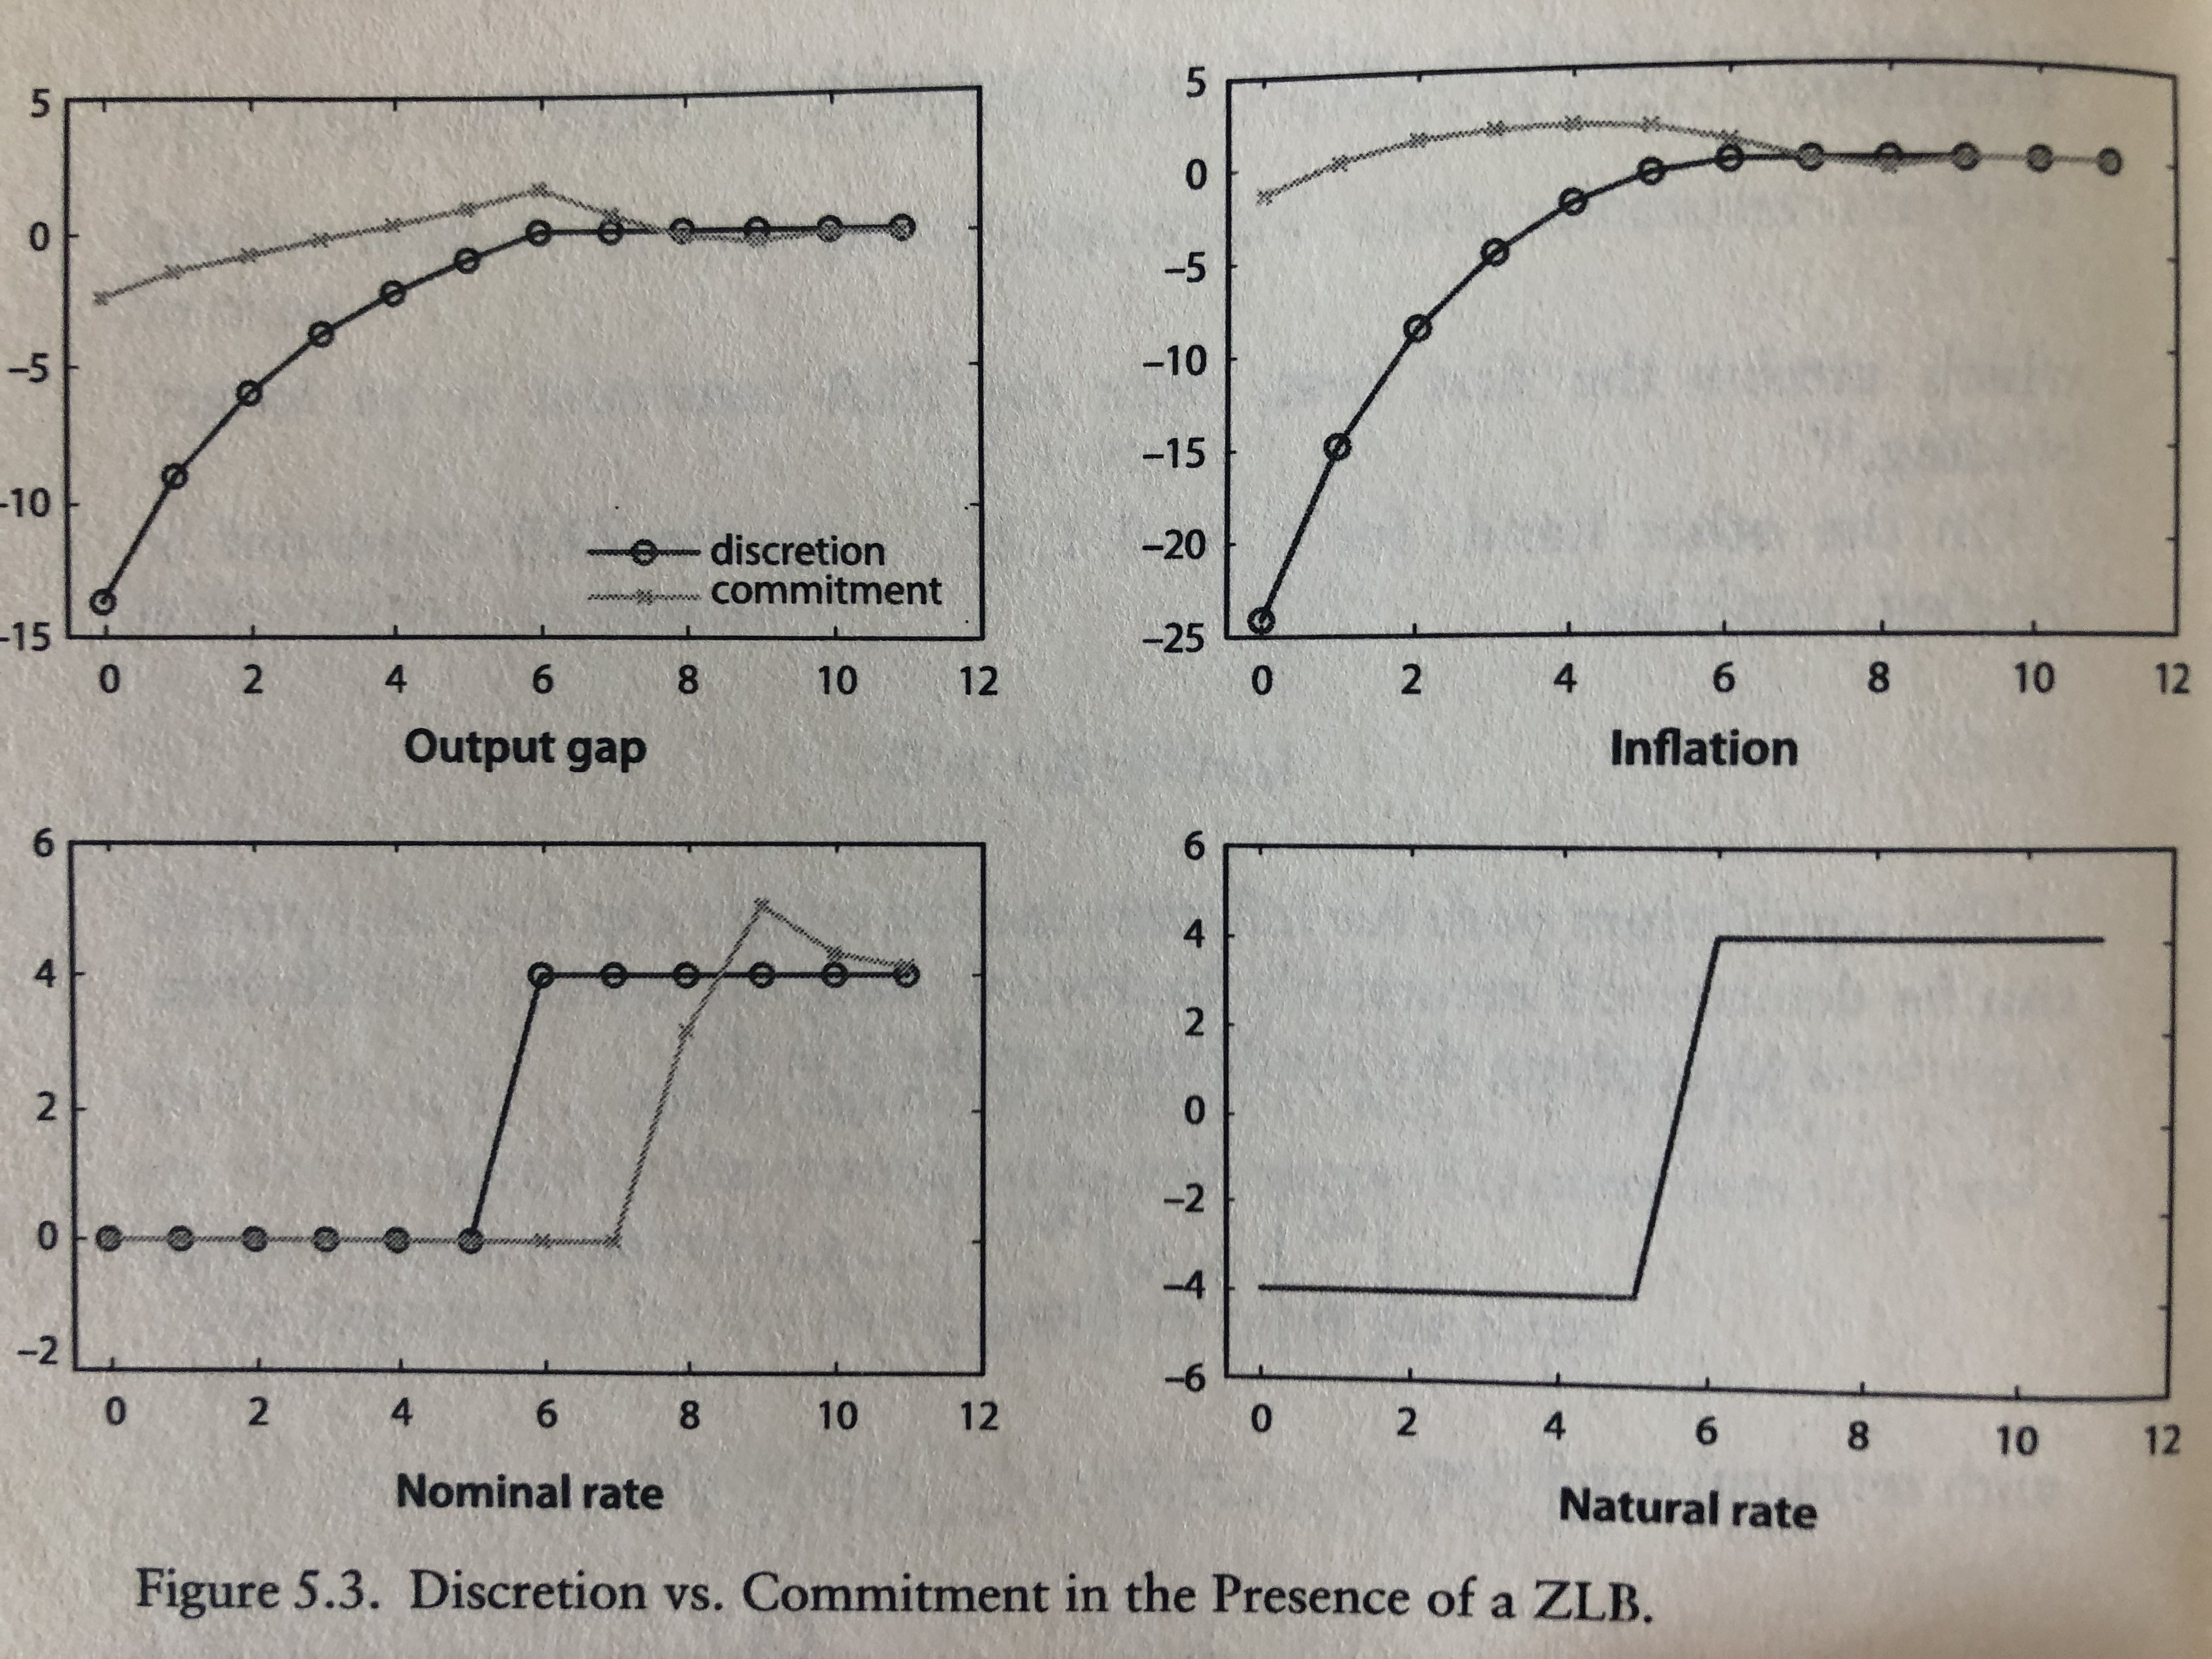
\includegraphics[scale=0.075]{../../Images/Gali2018irfZLB.jpeg}
\end{frame}


\begin{frame}
\frametitle{What Is the Effect of a Liquidity Trap in the NK Model?}
\begin{itemize}
	\item Why the big slump?
	\item Even if inflation were zero, consumption would be depressed by
	\begin{align*}
		\hat{x}_t &= -\sigma \sum_{s=0}^{T}\Delta  
	\end{align*}
	\begin{itemize}
		\item Households desired savings too high because $\hat{r}_{t+1}$ is too high.
	\end{itemize}
	\item Key Idea: Deflation exacerbates the ZLB.
	\begin{itemize}
		\item Deflation occurs because negative output gaps push down MC.
		\item This pushes $\hat{r}_{t+1}$ higher as $\hat{r}_{t+1} = -E_t\{\hat{\pi}_{t+1}\}$, which makes $\hat{x}_t$ lower, leading to more deflation....
		\begin{align*}
			\hat{x}_t &= -\sigma \sum_{s=0}^{T}(\Delta-\hat{\pi}_{t+s+1})	
		\end{align*}
		\item Inflation is forward looking, so deflation is worst at the beginning and then gets better.
	\end{itemize}
\end{itemize}
\end{frame}


\begin{frame}
\frametitle{The Paradox of Flexibility}
\begin{itemize}
	\item Would more flexible prices make things better?
	\begin{itemize}
		\item NO! Surprisingly, they make things worse!	
	\end{itemize}
	\item Output gap with perfectly sticky prices is:
	\begin{align*}
		\hat{x}_t &= -\sigma \sum_{s=0}^{T}\Delta  
	\end{align*}
	\item Output gap with flexible prices (larger $\kappa$) is:
	\begin{align*}
			\hat{x}_t &= -\sigma \sum_{s=0}^{T}(\Delta-\hat{\pi}_{t+s+1})	
		\end{align*}
		with $\hat{\pi}_{t+s+1}$ increasing as $\kappa\rightarrow\infty$.
	\item Intuition: Deflation is what turbocharges liquidity trap.
	\begin{itemize}
		\item More flexibility $\Rightarrow$ more deflation $\Rightarrow$ worse spiral.
	\end{itemize}
\end{itemize}	
\end{frame}

%%%%%%%%%%%%%%%%%%%%%%%%%%%%%%%%%%%%%%%%%%%%%%%%%%
\section{Monetary Policy at ZLB}
%%%%%%%%%%%%%%%%%%%%%%%%%%%%%%%%%%%%%%%%%%%%%%%%%%


\begin{frame}
\frametitle{What Is Optimal Monetary Policy in a Liquidity Trap?}
\begin{itemize}
	\item What does monetary policy want to do in a liquidity trap?
	\begin{itemize}
		\item $i_t=0 \Rightarrow$ It can't do anything!
	\end{itemize}
	\item But, as with optimal monetary policy, can gain from committing self to non-discretionary solution.
	\begin{itemize}
		\item This time with respect to policy \emph{after} the liquidity trap.
		\item In particular, it wants to \emph{commit to inflating}!
	\end{itemize}
\end{itemize}	
\end{frame}


\begin{frame}
\frametitle{What Is Optimal Monetary Policy in a Liquidity Trap?}
\begin{itemize}
	\item In T period liquidity trap with commitment:
	\begin{align*}
		\hat{x}_t &= -\sigma \sum_{s=0}^{T}(\Delta-\hat{\pi}_{t+s+1}) -\sigma \sum_{s=T+1}^{\infty}(\hat{i}_{t+s}-\hat{\pi}_{t+s+1}) \\
		\hat{\pi}_t&=\sum_{s=0}^{\infty}\beta^s \kappa \hat{x}_{t+s}
	\end{align*}
	\item Causing an inflationary boom when the liquidity trap is over:
	\begin{enumerate}[1.]
		\item Reduces ``over saving'' problem causing the trap.
		\begin{itemize}
			\item Boom in future, so less reason to save.
			\item This is the root cause. It would help even with fixed prices.
		\end{itemize}
		\item Reduces deflation $\Rightarrow$ mitigates deflationary spiral.
		\begin{itemize}
			\item Inflation today pushes $r_t$ down towards $r_{t}^{n}$.
		\end{itemize}
	\end{enumerate}
\end{itemize}	
\end{frame}


\begin{frame}
\frametitle{Central Bank Problem}
\begin{align*}
\min_{\hat{x}_{t+s},\hat{\pi}_{t+s}}\frac{1}{2}\sum_{s=0}^{\infty}&\beta^s\left(\hat{\pi}_{t+s}^2 + \vartheta \hat{x}_{t+s}^{2}\right) \\
	\text{s.t. }\hat{\pi}_t&=\beta \hat{\pi}_{t+1} +  \kappa \hat{x}_{t} \\
	\hat{x}_t &\le  \hat{x}_{t+1} -\sigma(-\rho-\hat{\pi}_{t+1}-\hat{r}_{t+1}^n) 
\end{align*}
\begin{itemize}
	\item Second constraint combines IS and ZLB ($i_t\ge 0 \Rightarrow \hat{i}_t \ge -\rho $)
	\item T-period liquidity trap as before:
	\begin{align*}
		\hat{r}_{t+1}^n =  \begin{cases} -\rho-\Delta<0 & \text{from } t \text{ to } t+T \\  0 & \text{from } t+T+1 \text{ onwards}\end{cases}
	\end{align*}
\end{itemize}	
\end{frame}


\begin{frame}
\frametitle{Central Bank Lagrangian}
\begin{align*}
\mathcal{L}=\frac{1}{2}\sum_{s=0}^{\infty}\beta^s\begin{bmatrix}\left(\hat{\pi}_{t+s}^2 + \vartheta \hat{x}_{t+s}^{2}\right)+\xi_{1,t+s}\left(\hat{\pi}_{t+s}-\beta \hat{\pi}_{t+s+1}-\kappa \hat{x}_{t+s}\right) \\
	+\xi_{2,t+s}\left(\hat{x}_{t+s} -  \hat{x}_{t+s+1} +\sigma(-\rho-\hat{\pi}_{t+s+1}-\hat{r}_{t+s+1}^n) \right)\end{bmatrix}
\end{align*}
\begin{itemize}
	\item FOCs:
	\begin{align*}
		\hat{\pi}_{t}+\xi_{1,t}-\xi_{1,t-1}-\frac{\sigma}{\beta}\xi_{2,t-1} &=0\qquad (\hat{\pi}_t) \\
		\vartheta\hat{x}_{t}-\kappa\xi_{1,t}+\xi_{2,t}-\frac{1}{\beta}\xi_{2,t-1} &=0\qquad (\hat{x}_t) 
	\end{align*}
	\item Complementary slackness conditions:
	\begin{align*}
		\xi_{2,t}\ge 0, \hat{i}_t\ge -\rho ,\xi_{2,t}(\hat{i}_t+\rho)=\xi_{2,t}i_t=0
	\end{align*}
\end{itemize}	
\end{frame}


\begin{frame}
\frametitle{Central Bank Commitment Solution}
\begin{itemize}
	\item Show positive output gap and inflation at $T+1$ by differencing FOCs for between $T+1$ and $T$ and using $\xi_{2,T+1}=0$:
	\begin{align*}
		\hat{x}_{T+1}-\hat{x}_{T}=-\frac{\kappa}{\vartheta}\hat{\pi}_{T+1}+\frac{\beta+\sigma\kappa}{\vartheta\beta}\xi_{2,T}+\frac{1}{\vartheta\beta}(\xi_{2,T}-\xi_{2,T-1}) 
	\end{align*}
	\begin{itemize}
		\item First term is standard leaning against the wind effect. If this alone, $\hat{x}_{T+1}=\hat{x}_{T}=\hat{\pi}_{T+1}=0$.
		\item Second two terms push towards positive growth since marginal value of relaxing constraint positive, $\xi_{2,T}>0$, which make you want to set $\hat{x}_{T+1}>0$.
		\item Asymptotically returns to $\hat{x}_t=\hat{\pi}_t=0$.
	\end{itemize}
	\item Intuition: Second order inflation and output gap loss in future, first order output gap and deflation gain today.
	\item Werning (2012) solves full dynamic path using continuous time methods, shows $\hat{i}_t =-\rho$ for $t\in[t,T_c]$ for $T_c>0$ and then jumps discretely.
\end{itemize}	
\end{frame}


\begin{frame}
\frametitle{Central Bank Commitment Solution}
\centering
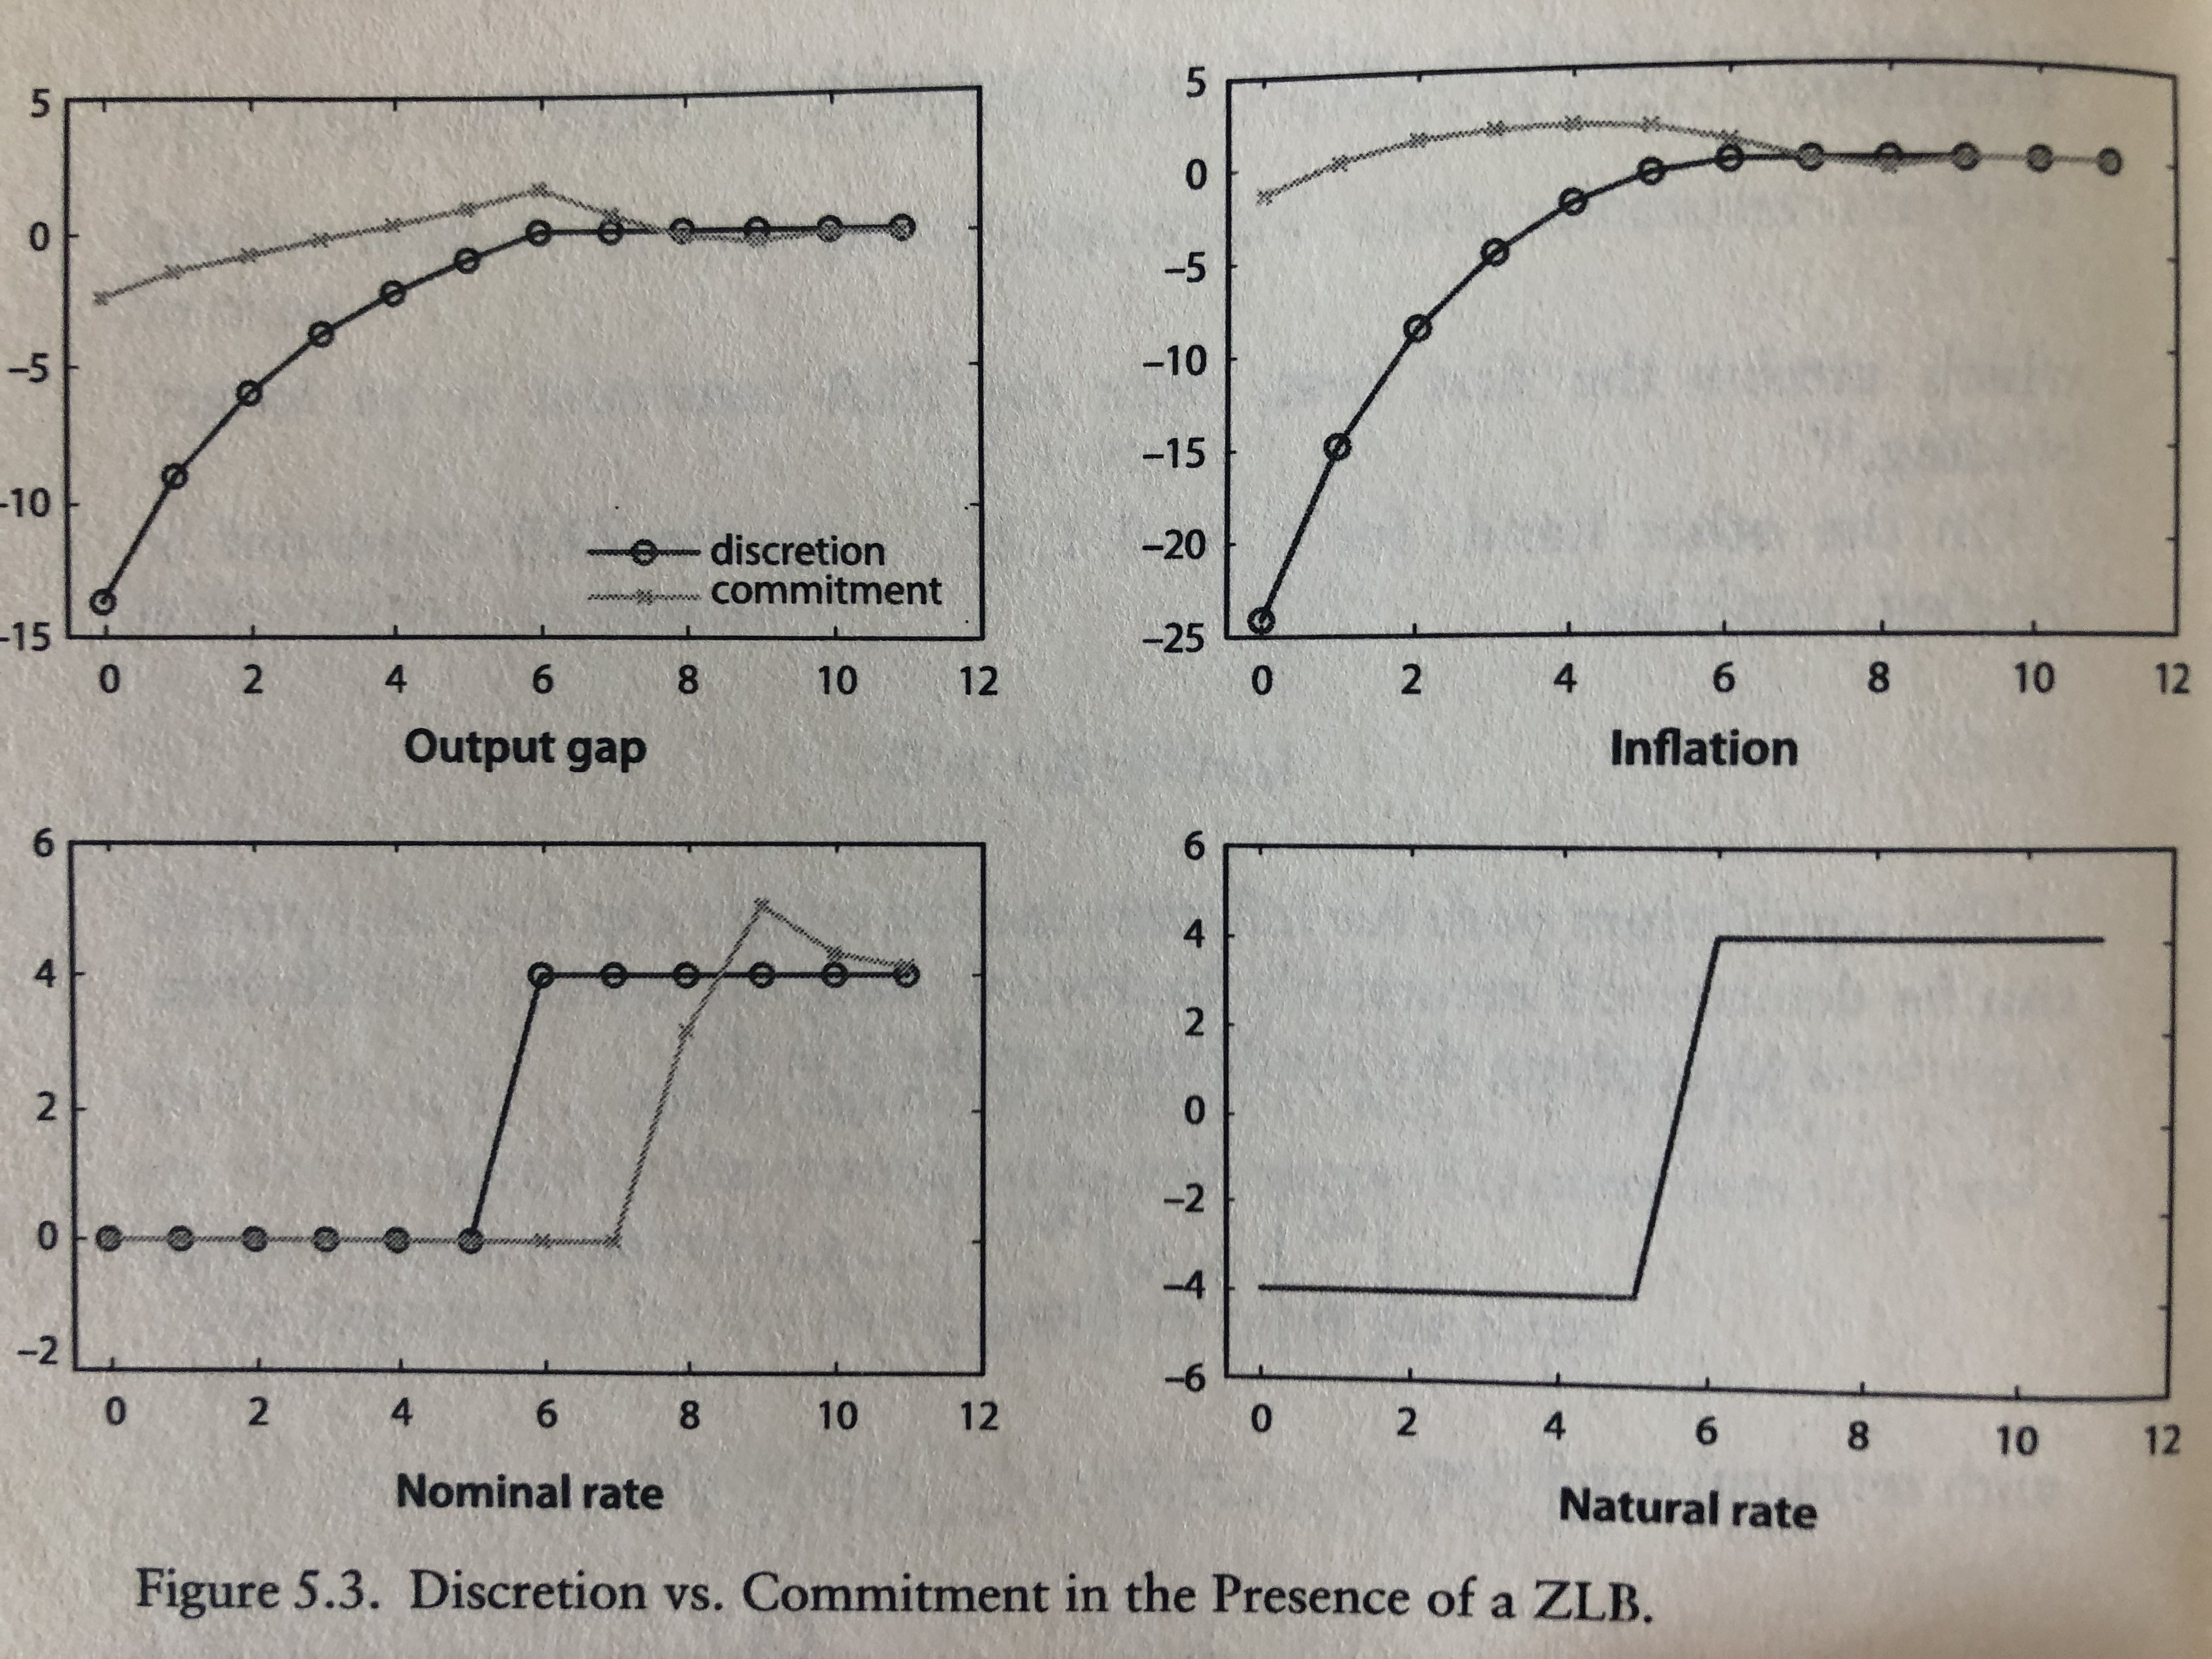
\includegraphics[scale=0.075]{../../Images/Gali2018irfZLB.jpeg}
\end{frame}


\begin{frame}
\frametitle{Central Bank Commitment Solution}
\begin{itemize}
	\item This commitment solution motivates \emph{forward guidance}.
	\begin{itemize}
		\item Announce you are going to keep your rate low for a long time, unconditional on market conditions.
		\item Idea: Get people to believe that you will keep rates low after the ZLB does not bind.
		\item Problem: Not a time consistent commitment.
		\item Also when do you know you are out? $T-$period trap is stylized and period of ending is endogenous.
	\end{itemize}
	\item Fed used forward guidance:
	\begin{itemize}
		\item In December 2008 says ``likely to warrant exceptionally low levels of the federal funds rate for some time.''
		\item In August 2011, introduce specific date stating that will be low through mid 2013.
		\item Pushed that out twice to late 2014 and mid-2015 in 2012.
	\end{itemize}
	\item Key empirical question: is the Fed following a commitment strategy or simply providing forecasts?
\end{itemize}	
\end{frame}

\begin{frame}
\frametitle{Forward Guidance Puzzle}
\begin{itemize}
	\item Promises of low future interest rates very effective in new Keynesian model at ZLB.
	\begin{itemize}
		\item Probably too effective.
		\item This is known as the ``forward guidance puzzle.''
	\end{itemize}
	\item Simple example:
	\begin{itemize}
		\item Promise low real rate $\hat{r}_{t+T}<0$, $T$ periods in the future.
		\item Fix nominal rate until then.
	\end{itemize}
\end{itemize}	
\end{frame}

\begin{frame}
\frametitle{Forward Guidance Puzzle}

\begin{itemize}
\item No further shocks, so return to steady state at $t+T+1$.
\begin{align*}
		\hat{x}_t &= \sigma \sum_{s=0}^{T}\hat{\pi}_{t+s+1} - \sigma \hat{r}_{t+T}  \\
		\hat{\pi}_t&=\sum_{s=0}^{T}\beta^s \kappa \hat{x}_{t+s}
	\end{align*}
	\begin{itemize}
		\item Low real rate raises all output gaps from $t$ to $t+T$ by $-\sigma \hat{r}_{t+T}$.
		\item Higher output gap means higher inflation.
		\item Real rate drops even more, further stimulating output.
		\item[$\Rightarrow$] ``Virtuous cycle'' of higher output and higher inflation.
	\end{itemize}
	\item Effect \emph{increases} the further away the promise is (higher $T$).
	\begin{itemize}
		\item Generally viewed as unreasonable.
		\item But difficult to test in practice.
		\item Key issue: is central bank able to commit to such a policy?
	\end{itemize}
\end{itemize}	
\end{frame}

\begin{frame}
\frametitle{Other Unconventional Policies}

\begin{itemize}
\item Fed also pursued \emph{Large-Scale Asset Purchases} (also known as ``quantitative easing'').
\item There is not just one short term rate.
	\begin{itemize}
		\item Fed Funds Rate
		\item Longer-maturity treasury rates.
		\item Checking interest / certificate of deposit rate.
		\item Mortgage rates.
		\item Business loan rates.
	\end{itemize}
	\item Other rates are usually spreads over FFR.
	\item By buying treasuries and GSE mortgage-backed securities, reduce spreads and interest rates for consumers and businesses.
	\begin{itemize}
		\item Much more difficult to assess these policies.
		\item Very few models are able to match macro data and term premia.
		\item And even fewer allow the Fed to influence these prices. Generally requires some limits to arbitrage.
	\end{itemize}
\end{itemize}	
\end{frame}

\begin{frame}
\frametitle{Optimal Inflation Rate?}

\begin{itemize}
\item Many of these policies are controversial.
\item Most controversial: raise the inflation target above 2\%.
	\begin{itemize}
		\item Benefits:
		\begin{enumerate}[1.]
			\item Helps us get out of liquidity trap now.
			\item In future, need $r_{t}^n < -\pi_t$ to fall in, so fall in less frequently.
		\end{enumerate}
	\item Olivier Blanchard floated 4\%. Nobody has yet adopted.	
	\item In macro-models low inflation rates tend to be optimal (Coibion, Gorodnichenko, Wieland, 2012).
	\begin{itemize}
		\item Pay cost of higher inflation every period, but gain benefit only in periods of ZLB.
		\item Suggest that more aggressive state-contingent policies, such as PLT, is preferred.
	\end{itemize}
	\item Practical circles worry about runaway inflation and that inflation expectations will become ``unanchored.''
	\item Unclear to what extent the Fed would even be able to raise the inflation rate (see Abenomics in Japan, U.S. after lift-off in 2015).
\end{itemize}
\end{itemize}	
\end{frame}


\begin{frame}
\frametitle{Is Zero the Lower Bound?}

\begin{itemize}
\item Recently, moved into a world of negative interest rates.
	\begin{itemize}
		\item Swiss, Swedes, Danish, ECB, and Japanese all have negative rates (for banks, not people).
	\item Get banks to lend money by taxing reserves and reducing other rates to zero.
	\end{itemize}
	\item Money demand has not exploded up yet.
	\begin{itemize}
		\item Clearly would if you go negative enough.
		\item But what is ``negative enough''? We really do not know..
	\end{itemize}
	\item See Rognlie (2016) for model where money demand explodes at negative rate rather than zero, but negative rates cause costly distortions.
	\item See Eggertsson et al. (2019) for evidence that the pass-through of policy rates to deposit rates breaks down when the policy rate becomes negative.
\end{itemize}	
\end{frame}


%%%%%%%%%%%%%%%%%%%%%%%%%%%%%%%%%%%%%%%%%%%%%%%%%%
\section{What Is the Role of Fiscal Policy in a Liquidity Trap?}
%%%%%%%%%%%%%%%%%%%%%%%%%%%%%%%%%%%%%%%%%%%%%%%%%%

\begin{frame}
\frametitle{Fiscal Policy in a Liquidity Trap}

\begin{itemize}
\item In 2009, passed ARRA (e.g., the ``Stimulus Act'').
\item In there a stronger case for fiscal stimulus at the ZLB?
	\begin{itemize}
		\item Is the multiplier higher?
		\item Other justification: $\hat{x}_t<0\Rightarrow$ marginal costs are low, so cheap for government to buy its goods now, and it is low so cheap for it to finance with bonds.
	\end{itemize}
	\item To answer multiplier question, first look at multiplier in normal times in standard NK model, then consider ZLB.
	\item Relatively little work on optimal monetary policy. Werning (2012) a rare and very useful exception.
\end{itemize}	
\end{frame}


\begin{frame}
\frametitle{Government Spending in New Keynesian Model}

\begin{itemize}
\item Assume government consumes $G_t$ and finances with lump sum taxes $T_t$ and bonds $B_t$:
\begin{align*}
	\frac{1}{R_{t+1}}B_{t+1}=B_t+G_t-T_t
\end{align*}
\item With perfect capital markets and no default
\begin{align*}
	B_t + \sum_{s=0}^{\infty}\frac{G_{t+s}}{\prod_{j=0}^s R_{t+1+j}} = \sum_{s=0}^{\infty}\frac{T_{t+s}}{\prod_{j=0}^s R_{t+1+j}}
\end{align*}
\item  Assume $G_t$ follows exogenous process.
\end{itemize}	
\end{frame}

\begin{frame}
\frametitle{Government Spending in New Keynesian Model}

\begin{itemize}
\item Household BC
\begin{align*}
	C_t &= \frac{W_t}{P_t}N_t+TR_t+PR_t-T_t-\frac{B_t-Q_{t-1}B_{t-1}}{P_t}-\frac{M_t-M_{t-1}}{P_t} \\
	&=\text{Income}_t - T_t - \frac{B_t-Q_{t-1}B_{t-1}}{P_t}-\frac{M_t-M_{t-1}}{P_t}
\end{align*}
where $\text{Income}_t=\frac{W_t}{P_t}N_t+TR_t+PR_t$.
\item Then present value BC is:
\begin{align*}
	B_t + M_t +\sum_{s=0}^{\infty}\frac{\text{Income}_{t+s}-T_{t+s}}{\prod_{j=0}^s R_{t+1+j}} = \sum_{s=0}^{\infty}\frac{C_{t+s}}{\prod_{j=0}^s R_{t+1+j}}
\end{align*}
and substituting government BC, Ricardian equivalence holds.
\begin{itemize}
	\item Timing of taxes does not matter.
	\item But changes in $G_t$ matter.
\end{itemize}
\end{itemize}	
\end{frame}


\begin{frame}
\frametitle{Equilibrium}
\begin{align*}
	\frac{W_t}{P_t}&=\frac{\chi N_t^\varphi}{C_t^{-\gamma}} \\
	1&=\beta E_t\left\{Q_t \frac{P_t}{P_{t+1}} \frac{C_{t+1}^{-\gamma}}{C_{t}^{-\gamma}}\right\}=E_{t}\{\Lambda_{t,t+1}R_{t+1}\} \\
	P_t&=\left[\theta P_{t-1}^{1-\epsilon} + (1-\theta) P_{t}^{*1-\epsilon}\right]^{\frac{1}{1-\epsilon}} \\
	P_t^* &=  (1+\mu)E_t\left\{\sum_{s=0}^{\infty}\frac{\theta^s\Lambda_{t,t+s}Y_{t+s}P_{t+s}^{\epsilon-1}}{\sum_{k=0}^{\infty}\theta^k\Lambda_{t,t+k}Y_{t+k}P_{t+k}^{\epsilon-1}}\frac{W_{t+s}}{A_{t+s}}\right\} \\
	Y_t&=C_t\color{red}+G_t\color{black} \\
Y_t&=A_tN_t\left[\int_0^1\left(\frac{N_t(i)}{N_t}\right)^{\frac{\epsilon-1}{\epsilon}}di\right]^{\frac{\epsilon}{\epsilon-1}} \\
	Q_t &= \beta^{-1}\left(\frac{P_t}{P_{t-1}}\right)^{\phi_{\pi}}\left(\frac{Y_t}{Y_t^{flex}}\right)^{\phi_{y}}e^{v_t}
\end{align*}	
\end{frame}


\begin{frame}
\frametitle{Log Linearized IS and Natural Rate}
\begin{itemize}
	\item Log-linearizing resource constraint gives
	\begin{align*}
		\hat{y}_t=\color{red}(1-s_g)\color{black}\hat{c}_t + \color{red}s_g \hat{g}_t\color{black}
	\end{align*}
	\item Log-linearizing Euler equation and plugging in
	\begin{align*}
		\hat{y}_t=-\color{red}(1-s_g)\color{black}\sigma\left(\hat{i}_t-E_t\{\hat{\pi}_{t+1}\}\right) + E_t\{\hat{y}_{t+1}\} + \color{red}s_g (\hat{g}_t-E_t\hat{g}_{t+1})\color{black}
	\end{align*}
	\item Consequently in the flex price equilibrium
	\begin{align*}
		\hat{y}_t^n=-\color{red}(1-s_g)\color{black}\sigma E_t\{\hat{r}_{t+1}^n\} + E_t\{\hat{y}_{t+1}\} + \color{red}s_g (\hat{g}_t-E_t\hat{g}_{t+1})\color{black}
	\end{align*}
	\item Difference gives modified IS curve:
	\begin{align*}
		\tilde{y}_t=-\color{red}(1-s_g)\color{black}\sigma E_t\left(\hat{i}_t-\hat{\pi}_{t+1}-\hat{r}_{t+1}^n\right) + E_t\{\tilde{y}_{t+1}\} 
	\end{align*}
	where:
	\begin{align*}
		\hat{r}_{t+1}^n = \frac{1}{\sigma\color{red}(1-s_g)\color{black}}\left(E_t\{\hat{y}_{t+1}^n\}-\hat{y}_t^n\right) + \color{red}\frac{s_g}{(1-s_g)\sigma} (\hat{g}_t-E_t\hat{g}_{t+1})\color{black}
	\end{align*}
\end{itemize}
\end{frame}


\begin{frame}
\frametitle{Flex Price Equilibrium}
\begin{align*}
	\hat{y}_t^n&=\hat{a}_t+\hat{n}_t^n \\
	\hat{y}_t^n-\hat{n}_t^n&=\varphi\hat{n}_t^n+\gamma\hat{c}_t^n \\
	\hat{y}_t&=\color{red}(1-s_g)\color{black}\hat{c}_t + \color{red}s_g \hat{g}_t\color{black}
%	-\varphi/\gamma \hat{y}_t^n +(1+\varphi)/\gamma\hat{a}_t &=\hat{c}_t^n \\
%	\gamma\hat{y}_t&=\color{red}(1-s_g)\color{black}(-\varphi \hat{y}_t^n +(1+\varphi)\hat{a}_t) + \color{red}\gamma s_g \hat{g}_t\color{black}
\end{align*}
\begin{itemize}
	\item Solve for output:
	\begin{align*}
		\hat{y}_t^n&=\left(\frac{1+\varphi}{\varphi+\frac{\gamma}{\color{red}(1-s_g)\color{black}}}\right)\hat{a}_t + \color{red}\frac{\gamma s_g}{(1-s_g)\varphi+\gamma} \hat{g}_t\color{black}
	\end{align*}
	\item Plug into natural rate of interest
	\begin{align*}
		\hat{r}_{t+1}^n = -\psi_a\left(E_t\{\hat{y}_{t+1}^n\}-\hat{y}_t^n\right) + \color{red}\psi_g(\hat{g}_t-E_t\hat{g}_{t+1})\color{black}
	\end{align*}
	where $\psi_a=\frac{\gamma(1+\varphi)}{\varphi\color{red}(1-s_g)\color{black}+\gamma}$ and $\psi_g=\frac{\gamma s_g \varphi}{(1-s_g)\varphi+\gamma} $
\end{itemize}
\end{frame}


\begin{frame}
\frametitle{Summary of Model With G}
\begin{align*}
		\tilde{y}_t &=-\color{red}(1-s_g)\color{black}\sigma E_t\left(\hat{i}_t-\hat{\pi}_{t+1}-\hat{r}_{t+1}^n\right) + E_t\{\tilde{y}_{t+1}\}  \\
		\hat{\pi}_t &= \kappa\tilde{y}_t+\beta E_t \{\hat{\pi}_{t+1}\} \\
		\hat{y}_t^n&=\left(\frac{1+\varphi}{\varphi+\frac{\gamma}{\color{red}(1-s_g)\color{black}}}\right)\hat{a}_t + \color{red}\frac{\gamma s_g}{(1-s_g)\varphi+\gamma} \hat{g}_t\color{black} \\
		\hat{r}_{t+1}^n &= -\psi_a\left(E_t\{\hat{y}_{t+1}^n\}-\hat{y}_t^n\right) + \color{red}\psi_g(\hat{g}_t-E_t\hat{g}_{t+1})\color{black} \\
		\hat{y}_t &= \tilde{y}_t + \hat{y}_t^n
	\end{align*}
\begin{itemize}
	\item Government spending affects $\hat{r}_{t+1}^n$ and $\hat{y}_{t}^n$
	\begin{itemize}
		\item Due to negative wealth effect from taxation increasing labor supply $\uparrow\hat{g}_t\Rightarrow \uparrow \hat{y}_t^n, \hat{r}_{t+1}^n$.
	\end{itemize}
\end{itemize}
\end{frame}


\begin{frame}
\frametitle{Government Spending Multiplier}
\begin{itemize}
	\item If the central bank sets $\hat{i}_t=\hat{r}_{t+1}^n+E_t\{\pi_{t+1}\}+\phi_{\pi}\hat{\pi}_t$, $\tilde{y}_t=0$ and $\hat{y}_t=\hat{y}_t^n$:
	\begin{align*}
		\frac{d\hat{y}_t}{d\hat{g}_t}=\frac{d\hat{y}_t^n}{d\hat{g}_t}=\frac{\gamma s_g}{(1-s_g)\varphi+\gamma}
	\end{align*}
	\item The multiplier is then:
	\begin{align*}
		\frac{dY_t}{dG_t}=\frac{Y}{G}\frac{d\hat{y}_t}{d\hat{g}_t}=\frac{\gamma}{(1-s_g)\varphi+\gamma}<1
	\end{align*}
	\item Government spending crowds out consumption.
	\begin{itemize}
		\item A \$1 of spending results in less than \$1 of output.
		\item Why? Increase in the real interest rate reduces consumption today through intertemporal subsitution.
		\item High real interest rate signals that resources are scarcer today, because the government takes them and throws them away.
	\end{itemize}
\end{itemize}
\end{frame}


\begin{frame}
\frametitle{Government Spending in a Liquidity Trap}
\begin{itemize}
	\item Return to $T-$period liquidity trap example with CB setting optimal discretionary policy:
	\begin{align*}
		\hat{y}_t &= -\sigma(1-s_g) \sum_{s=0}^{T}(-\hat{\pi}_{t+s+1}) \\
		\tilde{y}_t &= \hat{y}_t -\sigma(1-s_g) \sum_{s=0}^{T}(-\hat{r}_{t+1+s}^n) \\
		\hat{\pi}_t&=\sum_{s=0}^{T}\beta^s \kappa \tilde{y}_{t+s}
	\end{align*}
	\item \emph{Government spending has stimulative effect through inflation.}
	\begin{itemize}
		\item Government spending raises MC of production ($\propto \tilde{y}_t$), which raises inflation through NKPC.
		\item Higher expected inflation reduces real interest rate, which expands output today through intertemporal subsitution.
	\end{itemize}
	\item Large multipliers at ZLB in calibrated models (well above 1).
\end{itemize}
\end{frame}


\begin{frame}
\frametitle{Government in a Liquidity Trap}
\begin{itemize}
	\item Normal times $\Rightarrow$ use monetary policy (more nimble).
	\item ZLB $\Rightarrow$ use fiscal policy (monetary policy has hands tied and
has to make non-credible commitments).
	\item However, very large multipliers \emph{depend on inflationary effects of fiscal stimulus and intertemporal subsitution.}
	\begin{itemize}
		\item Is the mechanism credible?
	\end{itemize}
%	\begin{itemize}
%		\item Problem is ``too much saving'' and too little spending.
%		\item Government spending raises MC of production, improving output gap
%through agg demand effect even in absence of inflation effect.
%		\item High real interest rate signals that resources are scarcer today, because the government takes them and throws them away.
%	\end{itemize}
%	\item Large multipliers at ZLB in calibrated models (well above 1).
\end{itemize}
\end{frame}

%%%%%%%%%%%%%%%%%%%%%%%%%%%%%%%%%%%%%%%%%%%%%%%%%%
\section{All the Paradoxes}
%%%%%%%%%%%%%%%%%%%%%%%%%%%%%%%%%%%%%%%%%%%%%%%%%%

\begin{frame}
\frametitle{Productivity Shocks in a Liquidity Trap}
\begin{itemize}
	\item Return to $T-$period liquidity trap example with CB setting optimal discretionary policy:
	\begin{align*}
		\hat{y}_t &= -\sigma(1-s_g) \sum_{s=0}^{T}(-\hat{\pi}_{t+s+1}) \\
		\tilde{y}_t &= \hat{y}_t -\sigma(1-s_g) \sum_{s=0}^{T}(-\hat{r}_{t+1+s}^n) \\
		\hat{\pi}_t&=\sum_{s=0}^{T}\beta^s \kappa \tilde{y}_{t+s}
	\end{align*}
	\item \emph{Higher productivity has contractionary effect through inflation.}
	\begin{itemize}
		\item Temporary higher productivity reduces natural rate of interest because the MC of production falls.
		\item This lowers inflation through NKPC.
		\item Lower expected inflation increases real interest rate, which contracts output today through intertemporal substitution.
	\end{itemize}
\end{itemize}
\end{frame}

\begin{frame}
\frametitle{Supply Shocks in a Liquidity Trap}
\begin{itemize}
	\item Argument applies to any shock to MC.
	\begin{itemize}
		\item Productivity, willingness to work, minimum wage, unions, employment taxes, capital destruction, oil supply shocks...
	\end{itemize}
	\item Can write a paper for each of them!
	\item But empirical evidence does not support these predictions (Wieland, 2019):
	\begin{itemize}
		\item 2011 Earthquake in Japan contractionary.
		\item Oil supply shocks more contractionary at ZLB than in normal times.
	\end{itemize}
	\item Suggests inflation expectations mechanism not main driver in practice.
	\item Note: fiscal policy can still be powerful for other reasons.
\end{itemize}
\end{frame}

%%%%%%%%%%%%%%%%%%%%%%%%%%%%%%%%%%%%%%%%%%%%%%%%%%
\section{Where do we stand?}
%%%%%%%%%%%%%%%%%%%%%%%%%%%%%%%%%%%%%%%%%%%%%%%%%%

\begin{frame}
\frametitle{\emph{Quo Vadis} NK Model?}
\begin{itemize}
	\item New Keynesian model has problems in a liquidity trap, just like in normal times.
	\item But still the benchmark for analyzing policy.
	\begin{itemize}
		\item Some sensible-looking predictions.
		\item Can be used to understand central bank actions.
		\item No clear alternative.
	\end{itemize}	
	\item Recent work has focussed on two key areas of improving the model:
	\begin{enumerate}
		\item Menu costs models of pricing rather than Calvo.
		\begin{itemize}
			\item Relatively well-settled: suggests Calvo is reasonable approximation.
		\end{itemize}
		\item Incomplete markets rather than permanent-income representative-agent.
		\begin{itemize}
			\item More recent literature suggests old-Keynesian MPCs more important than intertemporal substitution.
			\item But policy lessons (so far) largely similar to NK model.
		\end{itemize}
	\end{enumerate}
\end{itemize}
\end{frame}

\begin{frame}
\frametitle{Retrospective: That's All!}
\begin{itemize}
	\item We have covered a lot of ground in the last ten weeks!
	\begin{enumerate}
		\item Real Business Cycles
		\item The New Keynesian Model
		\begin{enumerate}
			\item Empirical Motivation for Nominal Rigidity
			\item Money, Money Demand, and Output
			\item Monopolistic Competition and Markups
			\item Full New Keynesian Model
		\end{enumerate}
		\item Optimal Policy in a New Keynesian Framework
		\item The Liquidity Trap and Policy in a Liquidity Trap
	\end{enumerate}	
	\item Hope you found class interesting and relevant for understanding business cycles and economic policy!
	\begin{itemize}
		\item Will hopefully see you around building soon.
		\item Good luck on exam and the rest of first year!
	\end{itemize}
\end{itemize}
\end{frame}

\end{document}